\documentclass[../proyecto.tex]{memoir}

\begin{document}

\chapter{Metodología}

Antes de continuar con la implementación y exposición de la técnica de simulación Monte Carlo es necesario introducir un marco teórico matemático que nos servirá de referencia además de establecer una base de trabajo concisa. Los formalismos nos permitirán articular la intuición de asincronismo en el esquema de actualización del autómata celular, cuyo homónimo biológico sería el procesamiento imperfecto de información entre individuos a causa de perturbaciones derivadas del medio o de la interacción con otros individuos. En este trabajo nos restringimos a un caso simple de asincronismo en la actualización: examinaremos que ocurre si todas las transiciones ocurren al mismo tiempo pero los individuos reciben la información del estado de sus vecinos de forma imperfecta.

En primer lugar introduciremos los conceptos básicos de teoría de conjuntos, probabilidad, computación y generación de números aleatorios sobre los que desarrollaremos las estimaciones Monte Carlo. Las claves de este desarrollo serán el teorema central del límite y la ley de los grandes números que esencialmente justifican la efectividad del método Monte Carlo. Continuaremos con la exposición del autómata celular m-asíncrono, el juego de vida de Conway $\alpha$-asíncrono y su representación,mostraremos las principales categorías de configuraciones iniciales y finalmente expondremos que criterio utilizaremos para intentar caracterizar el comportamiento de nuestras simulaciones.

\section{Teoría de conjuntos}

\subsection{Introducción}

Nos gustaría poder plasmar la intuición de que una célula tenga la misma probabilidad de ser actualizada independientemente o no del resto de células actualizadas en cada instante de tiempo. El concepto de ultrafiltro nos permitirá establecer una clase de autómata celular lo suficientemente general como para abarcar los nuevos tipos de autómatas celulares que introduciremos en posteriores secciones. 

Dado un conjunto X, $P(X)$ denota el conjunto de todos los subconjuntos de X. Dado $A \in \mathcal{P}(X)$, notaremos su complementario $A^{c}$. 
\begin{defi}
Un ultrafiltro de X es $U \in \mathcal{P}(X)$ tal que:

\begin{enumerate}
\item $\emptyset \in U$.
\item Sean $A,B \in \mathcal{P}(X)$ tales que $A \subset B$ y $ A \in U$, entonces $B \in U$.
\item Si $A,B \in U$, entonces $A \cap B \in U$.
\item Si $A \in \mathcal{P}(X)$ entonces o bien $A \in U$, o bien $ A^{c} \in U$.
\end{enumerate}

Además dado $p \in X$, el ultrafiltro $U_{p}$ diremos que es principal si es el más pequeño que contiene a $p$, esto es, la colección de todos los conjuntos que contienen a $p$.
\end{defi}

\section{Teoría de la probabilidad: conceptos básicos}

El contenido de esta sección está extraído de los siguientes textos en orden de empleo: \cite{elLibro, grandesNumeros, loeve}. 

\begin{defi}
Una $\sigma$-álgebra, $\mathds{F}$, sobre un conjunto $X$, es una colección no vacía de subconjuntos de $X$ cerrados para uniones numerables y para la operación de complementario, esto es:
\begin{itemize}
\item $\forall A \in \mathds{F}$ se verifica que $A^{c} \in \mathds{F}$.
\item $ \forall A_{n} \in \mathds{F}, n \in \mathds{N} $ se verifica que $\bigcup _{n \in \mathds{N}} A_{n} \in \mathds{F}$.
\end{itemize}
\end{defi}

\begin{defi}
Sean un conjunto $X$ con su $\sigma$-álgebra asociada, $\mathds{F}$, el par $(X, \mathds{F})$ es un espacio medible. 
\end{defi}

\begin{defi}
Una función medible es una función entre espacios medibles, $g: (X, \mathds{F}) \rightarrow (X', \mathds{F}')$ tal que: $g^{-1}(A) \in \mathds{F} \quad \forall A \in \mathds{F}'$.
\end{defi}

\begin{defi}
La tupla $(X, \mathds{F}, P)$ es un espacio de probabilidad si:
\begin{itemize}
\item $X$ es el espacio de muestreo, esto es, algún conjunto no vacío.
\item $\mathds{F}$ es una $\sigma$-álgebra de sucesos.
\item $P: \mathds{F} \to \mathds{R}$ es una medida de probabilidad, 
esto es, $P$ satisface los siguientes axiomas de Kolmogorov:
\begin{enumerate}
\item Para cada $A\in\mathds{F}$, existe un número $P(A) \geq 0$, esto es, la probabilidad del suceso $A$,
\item $P(X)=1$.
\item Sean ${A_n, n \geq 1}$ disjuntos, entonces: $$
	P \left( \bigcup_{n=1}^{\infty} A_{n} \right) = \sum_{n=1}^{\infty} P(A_n).
$$
\end{enumerate}
\end{itemize}
\end{defi}

\begin{defi}
Los sucesos ${A_n, n \geq 1}$ son independientes si y solo si $$
P \left( \bigcap_{n \geq 1} A_{n} \right) = \prod_{n \geq 1} P(A_n).
$$
\end{defi}

\begin{defi}
Un conjunto $A$ es abierto si, para cada punto $x\in A$, existe una bola de centro el punto y radio $\epsilon > 0$, $B(x,\epsilon)=\{ z : \abs{z-x} < \epsilon\}$, tal que $B(x,\epsilon) \subset F$. Así la $\sigma$-álgebra de Borel, es aquella generada por los conjuntos abiertos de $\mathds{R}$.
\end{defi}

De ahora en adelante supondremos que se ha fijado el espacio medible dado por $X=\mathds{R}$ y $F=\mathds{B}$ la $\sigma$-álgebra de Borel sobre $\mathds{R}$.

\subsection{Variables aleatorias}

\begin{defi}
Una variable aleatoria definida sobre un espacio de probabilidad $(X, \mathds{B}, P)$ es una función medible $A: X \to \mathds{R}$.
\end{defi}

Cada valor de $A$ se corresponde con un subconjunto de puntos de $X$ que se aplica en dicho valor: $\{ w\in X : A(w)=x\}$, que notaremos por simplicidad $\{X = x\}$. A parte de los anteriores conjuntos también nos resultarán de interés lo siguientes:
\begin{align*}
\{ w\in X : A(w) \leq x\} = \{ A \leq x \} \\
\{ w\in X : A(w) < x\} = \{ A < x \} \\
\{ w\in X : A(w) > x\} = \{ A > x \} \\
\{ w\in X : A(w) \geq x\} = \{ A \geq x \}
\end{align*}
%Con esta útil notación podremos notar fácilmente la probabilidad de sucesos de mayor interés.

\begin{prop} \label{funcion_de_va}
Si $g:\mathds{R}\to\mathds{R}$ es una función real de variable real, medible y $A$ es una variable aleatoria entonces $A'=g(A)$ es una variable aleatoria.
\end{prop}

\begin{defi}
La variables aleatorias $A_1, A_2,..., A_n$ son independientes si y solo si, para arbitrarios conjuntos de la $\sigma$-álgebra de Borel $B_1, B_2,..., B_n$: $$
	P \left( \bigcap_{k = 1}^{n} \{A_k \in B_k\} \right) = \prod_{k = 1}^{n} P(A_k \in B_k).
$$
\end{defi}

\begin{defi}
Dada una variable aleatoria $A$ se define su función de distribución como $ F : \mathds{R} \to [0,1] $ dada por:
$$
x \mapsto F(x)=P(A \leq x).
$$
\end{defi}

\begin{prop}
La función de distribución de la variable aleatoria $A$ satisface:
\begin{itemize}
\item Es monótona no decreciente.
\item Dada una sucesión decreciente de elementos de $\mathds{R}$, $\{x_n\}_{n \in \mathds{N}} \in \mathds{R}$ convergente a $x\in \mathds{R}$ se tiene $\lim_{x_n \to x} F(x_n) = F(x)$, es decir, es continua a la derecha.
\item $\lim_{x\to+\infty} F(x) = 1$ y $\lim_{x\to-\infty} F(x) = 0$.
\end{itemize}
\end{prop}

\begin{defi}
Sea $F$ una función de distribución definimos la función de densidad como la función integrable, $f$, tal que:
$$
F(b)-F(a) = \int^{b}_a f(x) dx, \quad \forall a < b. 
$$
\end{defi}

\begin{defi}
Sea $A$ una variable aleatoria, definimos su valor esperado o esperanza como sigue:
$$
\mathds{E}(A) = \int_{X}A(w)dP(w).
$$
Adicionalmente si $\mathds{E}\abs{A} < \infty$, diremos que $A$ es integrable.
\end{defi}

\begin{defi}
Sea una variable aleatoria $A$, definimos:
\begin{itemize}
\item Los momentos de orden $n$ de $A$: $\mathds{E}(A^n) = \int_{X}A(w)^{n}dP(w), \quad n \in \mathds{N}$.
\item Los momentos centrados de orden $n$ de $A$: $\mathds{E}_c(A^n) = E( (A-E(A))^n ), \quad n \in \mathds{N}$.
\end{itemize}
\end{defi}

Notar que los momentos no existen necesariamente para todo $n\in \mathds{N}$.

\begin{defi}
Definimos la varianza de la variable aleatoria $A$ con esperanza $\mu < \infty$ y $\mathds{E}_c(A^2) < \infty $ como:$$
var(A) \equiv \mathds{E}_c(A^2) = \mathds{E}(A^2) - \mu^2.
$$
\end{defi}

\begin{defi}
A la raíz cuadrada positiva de la varianza la notaremos $\sigma(A)=+\sqrt{var(A)}$ y diremos que es la desviación estándar de la variable aleatoria A. 
\end{defi}

\begin{prop}
Sea $A$ una variable aleatoria con esperanza $\mu < \infty$ y varianza $\sigma^2 < \infty$ y sea $A'=aA+b$, donde $a,b\in\mathds{R}$, entonces: $$
\mathds{E}(A')=a\mu + b \quad y \quad var(A') = a^2 \sigma^2.
$$

\end{prop}


\subsection{Variables aleatorias discretas}

\begin{defi}
Una variable aleatoria $A$ diremos que es discreta si toma valores es un conjunto numerable, esto es, $\exists E=\{x_n\}_{n \in \mathds{N}} \subset \mathds{R}$ tal que $P(A \in E)=1$. 
\end{defi}

\begin{defi}
La función de distribución de una variable aleatoria discreta $A$ es la siguiente: $$
\forall x\in \mathds{R}, \quad F(x) = P( A \leq x) = \sum_{x_n\in E, x_n \leq x} P(A=x_n).
$$
\end{defi}

\begin{defi}
Sea una variable aleatoria discreta $A$, definimos:

\begin{itemize}
\item Los momentos de orden $n$ de $A$: $\mathds{E}(A^n) = \sum_{x_m \in E} x_m^n P(A=x_m)$.
\item Los momentos centrados de orden $n$ de $A$: $\mathds{E}_c(A^n) =\sum_{x_m \in E} (x_m - \mu)^n P(A=x_m)$.
\end{itemize}
\end{defi}

El momento $n=1$ se conoce como valor esperado o esperanza: $$
\mathds{E}(A) \equiv \sum_{x_m \in E} x_m P(A=x_m).
$$

\begin{defi}[Tipos de convergencia: convergencia en probabilidad, convergencia casi segura y convergencia en distribución]
Sean ${A_n}$ ,$n\in \mathds{N}$ y $A$ variables aleatorias, definimos:
\begin{itemize}
\item $A_n \to A$ en probabilidad, si para todo $\epsilon > 0$, $\lim_{n\to\infty} P( |A_n-A|> \epsilon ) = 0$ y lo notaremos $A_n \to^{P} A$.
\item $A_n \to A$ casi seguramente, si $P(\lim_{n\to\infty} A_n=A) = 1$ y lo notaremos $A_n \to^{c.s.} A$.
\item $A_n \to A$ en distribución, si $\lim_{n \to \infty} P(A_n \leq x) = P(A \leq x),\quad \forall x \in \mathds{R}$ donde $x\mapsto P(A \leq x)$ es una función continua y lo notaremos $A_n \to^{d} A$.
\end{itemize}
\end{defi}

\begin{defi}
Sea $i$ el número completo $i=\sqrt{-1}$, la extensión de la función exponencial $exp: \mathds{R} \to \mathds{R^{+}}$ al cuerpo de los números complejos es $exp: \mathds{C} \to \mathds{C}$ dada por:
$$
z \mapsto exp(iz) = e^{iz}=\cos z+i\sin z.
$$
\end{defi}

Notar que el módulo de la exponencial compleja está acotado por la unidad :

$$
\abs{ exp(iz) } = \abs{\cos z+i\sin z} = \sqrt{\cos^2 z + \sin^2 z} = 1.
$$

Esta propiedad de la exponencial compleja nos asegura la existencia para toda variable aleatoria de la siguiente definición.

\begin{defi}
La función característica asociada a la variable aleatoria $A$ es la función $\phi_{A}: \mathds{R} \to \mathds{C}$, dada por:
$$
\phi_{A}(t) = \mathds{E}(e^{itA}).
$$
\end{defi}

\begin{prop}
Sea $\phi_A$ la función característica de la variable aleatoria $A$, entonces:

\begin{itemize}
\item $\abs{\phi_A(t)} \leq \phi_A(0)=1$.
\item $\phi_A$ es una función uniformemente continua.
\item $\phi_{cA+b}(t)=e^{itb}\phi_A(ct), \quad c,b\in \mathds{R}$.
\item Sea $A_1, A_2,...,A_n, n\in\mathds{N}$ una sucesión finita de variables aleatorias independientes, entonces: $$ 
\phi_{\sum^{n}_{i=1} A_i} (t) = \prod_{i=1}^{n} \phi_{A_i} (t) .
$$ Además si $A_1, A_2,...,A_n$ son idénticamente distribuidas: $$
\phi_{\sum^{n}_{i=1} A_i} (t) = \left( \phi_{A_1}(t) \right)^{n}.
$$
\item Si $\mathds{E}(A^k) < \infty$ su derivada k-ésima evaluada en 0 es $\phi_A^{(k)}(0)=i^k\mathds{E}(A^k)$.
\end{itemize}

\end{prop}

\subsection{Distribución normal}

\begin{defi} \label{normal}
Diremos que una variable aleatoria $A$ sigue una distribución normal con media $\mu < \infty$ y varianza $\sigma^2 < \infty$, $N(\mu,\sigma^2)$, si $A$ tiene la siguiente función de densidad: 

$$
f(x) = \frac{1}{ \sigma \sqrt{ 2 \pi }} exp \left( -\frac{1}{2}\left( \frac{x-\mu}{\sigma} \right)^2 \right),\quad \forall x \in \mathds{R}.
$$

Además su función característica es: $$
 \phi_{A}(t)=e^{-\frac{t^2}{2}}.
$$
\end{defi}

\section{Teoría de la probabilidad: teorema central del límite}

\begin{teorema} \label{central}
Sean $A_{1},A_{2},...,A_{n}$ variables aleatorias independientes, con esperanza $\mu < \infty$, varianza $\sigma^2 < \infty$ e idénticamente distribuidas. Entonces: $$
\frac{ \frac{1}{n}\sum_{i=1}^nA_i - n\mu}{ \sigma \sqrt{n}} \to^d N(0,1).
$$
\end{teorema}

Previa a la demostración del teorema central del límite, introducimos las herramientas matemáticas que nos harán posible su demostración.

\begin{teorema}[Teorema de Taylor]

Sea $k \in \mathds{N}$ y $f: \mathds{R} \to \mathds{R}$ k-veces diferenciable en el punto $a \in \mathds{R}$. Entonces existe una función $h_k: \mathds{R} \to \mathds{R}$ tal que:

$$
f(x)=f(a)+f'(a)(x-a)+\frac{f''(a)}{2!}(x-a)^2+\dotsb+\frac{f^{(k)}(a)}{k!}(x-a)^k + h_k(x)(x-a)^k
$$

y $\lim_{x\to a} h_k(x) = 0$.
\end{teorema}

\begin{teorema}[Teorema de continuidad] \label{cont}
Sean $A_1, A_2,...,A_n, n\in\mathds{N}$ variables aleatorias entonces: $$
\lim_{n \to \infty }{\phi_{A_n}} = \phi_{A}(t), \quad \forall t\in \mathds{R},
$$
si y solo si $$
A_n \to^d A.
$$

\end{teorema}

\begin{proof}[Demostración (Teorema central del límite)]

Sean $A_{1},A_{2},...,A_{n}$ variables aleatorias independientes idénticamente distribuidas con esperanza $\mu < \infty$ y varianza $\sigma^2< \infty$.
Sea ahora $$
Z_{n} = \frac{A_{1}+A_{2}+...+A_{n}-n\mu }{\sigma \sqrt{n}}.
$$
Definimos una nueva variable aleatoria, $Y_i$, que es la versión normalizada de $A_i$:$$
Y_i=\frac{A_i-\mu}{\sigma}
$$
Así definida, $Y_i$ es idénticamente distribuida con esperanza y varianza: $$
E(Y_{i}) = 0,  Var(Y_{i})=1.
$$
Sea ahora $Z_n = \frac{Y_1+Y_2+...+Y_n}{\sqrt{n}}$, queremos ver que: $$
\lim_{n \to \infty} \phi_{Z_{n}}(t)=e^{-\frac{t^{2}}{2}}.
$$

Procedemos a desarrollar el siguiente término:

$$
\phi_{\frac{Y_1+Y_2+...+Y_n}{\sqrt{n}}}(t) = \prod_{i=1}^{n} \phi_{\frac{Y_i}{\sqrt{n}}} (t) = \big(\phi_{\frac{Y_1}{\sqrt{n}}}(t) \big)^n.
$$

Aplicando el teorema de Taylor para obtener el desarrollo centrado en 0 para $k=2$ de $\phi_{Y_1}(\frac{t}{\sqrt{n}})$: 

\begin{align*}
\phi_{\frac{Y_1}{\sqrt{n}}}(t) &= \phi_{Y_1}(\frac{t}{\sqrt{n}}) \\
  &= \phi_{Y_1}(0) + \frac{t}{\sqrt{n}}\phi_{Y_1}^{'}(0) + \frac{t^2}{2n}\phi_{Y_1}^{''}(0) + \frac{t^2}{n} h_2(t)\\
 &= 1 + i\frac{t}{\sqrt{n}}\mathds{E}(Y_1) - \frac{t^2}{2n}\mathds{E}(Y_1^2) + \frac{t^2}{n} h_2(t)\\
 &= 1 + 0 - \frac{t^2}{2n} + \frac{t^2}{n} h_2(\frac{t}{\sqrt{n}}),
\end{align*}
donde $\lim_{t\to 0} h_2(\frac{t}{\sqrt{n}}) = 0$.

Obtenemos que: $$
\big(\phi_{Y_1}(\frac{t}{\sqrt{n}}) \big)^n =\big( 1 - \frac{t^2}{2n} + \frac{t^2}{n} h_2(\frac{t}{\sqrt{n}}) \big)^n\longrightarrow e^{-\frac{t^2}{2}}.
$$

cuyo límite es la función característica de una variable aleatoria perteneciente a una distribución normal con media 0 y varianza 1, concluimos la demostración aplicando el teorema de continuidad \ref{cont}.
\end{proof}

\section{Teoría de la probabilidad: ley de los grandes números}
\begin{teorema} \label{teo_grandes_numeros}
Sean $A_n$, $n \in \mathds{N}$ variables aleatorias independientes, con esperanza $\mu < \infty$ e idénticamente distribuidas. Entonces el valor medio de $A_n$, $\bar{\mu}$, converge casi seguramente a $\mu$:

$$
\bar{\mu}=\frac{1}{n}\sum_{n\in\mathds{N}} A_n \to^{c.s.} \mu,
$$

esto es, $P(\lim_{n\to\infty} \bar{\mu}=\mu) = 1$.

\end{teorema}

Para obtener una demostración un tanto más breve de éste teorema añadiremos la hipótesis de existencia del momento de orden 4 de $A_n$. Una demostración completa del teorema sin la hipótesis adicional se puede consultar en \cite{elLibro}.

\begin{lema}  \label{intercambio_suma}
Sean $A_n$,$ n \geq 1$ variables aleatorias no negativas, entonces: $$
E \left( \sum_{n \geq 1} A_n \right) = \sum_{n \geq 1} E(A_n).
$$

\end{lema}

\begin{lema}
En las misma condiciones de la ley de los grandes números, existe una constante $ K < \infty $ tal que para todo $ n \geq 0$:
$$
\mathds{E} \big( ( \bar{ \mu } - n \mu ) ^ 4 \big) \leq K n^2.
$$
\end{lema}

\begin{proof}

Sean 
$$
Z_k = A_k - \mu \quad y \quad T_n = Z_1 + Z_2 + ... + Z_n = \sum_{i=1}^{n} A_n - n\mu. 
$$

Entonces:

$$
\mathds{E} ( T_{n}^{4} ) = \mathds{E} ( \big( \sum_{i=1}^{n} Z_i \big) ^{4} ) = n\mathds{E}(Z_{1}^4)+3n(n-1)\mathds{E}(Z_1^2 Z_2^2) \leq Kn^2.
$$

donde en la segunda igualdad se ha empleado el desarrollo multinomial:

$$
(x_1+x_2+...+x_m)^n = \sum_{k_1+k_2+...+k_m=n} { n \choose k_1,k_2, ..., k_n} \prod_{1 \leq t \leq m} x_t^{k_t},
$$

con

$$
{ n \choose k_1,k_2, ..., k_n} = \frac{n!}{k_1!k_2! \dotsb k_n!}.
$$

Dado que $\mathds{E}(Z_k)=0 \quad \forall k$ y la independencia de las variables $Z_k$, se cancelan todos los sumandos de la forma:

\begin{align*}
	\mathds{E} (Z_{i} Z_{j}^3 ) &=\mathds{E} (Z_{i}) \mathds{E} (Z_{j}^3) = 0, \quad 1 \leq i,j \leq n, \quad i \neq j, \\
	\mathds{E} ( Z_{i} Z_{j} Z_{k} Z_{l} ) &= \mathds{E} (Z_{i}) \mathds{E} (Z_{j}) \mathds{E} (Z_{k}) \mathds{E} (Z_{l}) = 0, \quad 1 \leq i,j,k,l \leq n, \quad i \neq j \neq k \neq l.
\end{align*}

y siendo $K$ adecuadamente elegida, por ejemplo $K = 4 max{\mathds{E}(Z_1^4), \mathds{E}(Z_1^2)^2}$.
\end{proof}

Ya tenemos todos los rudimentos necesarios para proceder a demostrar el teorema de esta sección.

\begin{proof}[Demostración (Ley de los grandes números)]

Asumamos que $\mathds{E}_c( A_n^4) < \infty \quad \forall n$, aplicando el lema anterior:

$$
	\mathds{E} \big( ( \bar{ \mu } - \mu ) ^ 4 \big) \leq \frac{K}{n^{2}}.
$$

Ahora sea $Y_n = ( \bar{ \mu } - \mu ) ^ 4, \forall n \in \mathds{N}$ una variable aleatoria por la proposición \ref{funcion_de_va} y en particular es no negativa, luego podemos aplicar el lema \ref{intercambio_suma} en la siguiente cadena de igualdades:

$$
	\mathds{E} \big( \sum_{n \geq 1}( \bar{ \mu } - \mu ) ^ 4 \big) = \sum_{n \geq 1} \mathds{E} \big( ( \bar{ \mu } - \mu ) ^ 4 \big)  \leq K\sum_{n \geq 1}\frac{1}{n^{2}} < \infty,
$$

lo que implica:

$$
\abs{ \sum_{n \geq 1} \big( \bar{ \mu } - \mu \big)^ 4 } = \sum_{n \geq 1} \big( \bar{ \mu } - \mu \big)^ 4 < \infty \quad c.s. 
$$

Pero si una serie es convergente, entonces la sucesión de su término general de la serie converge a cero, por tanto:
$$
 \bar{ \mu } \to \mu \quad c.s.
$$
\end{proof}


\section{Generadores de números aleatorios}

Los generadores de números aleatorios no generan números realmente aleatorios, es decir, no son variables aleatorias idénticamente distribuidas. Dado un valor de inicialización de la secuencia o semilla generan siempre la misma sucesión de números, por tanto diremos que un generador de números aleatorios produce una secuencia indistinguible de una realmente aleatoria. Dicho ésto, podemos afirmar que un ordenador solo es capaz de generar secuencias de números pseudoaleatorios con un periodo de longitud finita.

Curiosamente, en las definiciones de los métodos de Monte Carlo no hay referencia explícita al empleo de la capacidades de cómputo de los ordenadores, sin embargo el gran desarrollo que han experimentado éstos desde el último tercio de siglo XX hasta nuestros días, los ha convertido en herramientas indispensables en las simulaciones Monte Carlo. La generación de números aleatorios ha experimentado también un importante crecimiento en las últimas décadas. Un tipo generador de números aleatorios muy usado venía dado por la siguiente ecuación recurrente:

\begin{equation} \label{cong}
I_{j+1} = aI_{j} +c \mod (m)
\end{equation}

donde $a$ es un entero positivo llamado multiplicador y $c$ es un número natural llamado incremento. Para $c \neq 0$, \ref{cong} es conocido por el nombre: \textit{generador lineal congruente de números aleatorios}. Claramente, en $n<m$ pasos la ecuación comienza a generar valores duplicados en el mismo orden, conocido ésto, se hacían elecciones particulares de $a,c$ y $m$ que obtuvieran en mayor periodo posible. En \cite{knuth} podemos encontrar algunos resultados notables sobre la elección parámetros $a,c$ y $m$. La elección del valor inicial $I_{0}$ no es relevante, pues se generarán todos los naturales posibles entre $0$ y $m-1$ antes de la primera repetición. Sin embargo no es suficiente con generar una sucesión de números de un largo periodo, además deben superar rigurosas baterías de test empíricos que aseguren una buena distribución de las secuencias de números además de la ausencia de patrones en las mismas. En el caso de los generadores lineales congruentes existe un resultado que afirma que las sucesivas n-tuplas de valores generados residen en al menos $(n!m)^\frac{1}{m}$ hiperplanos paralelos \cite{marsagliaRandom}, luego esta clase de generadores no son adecuados para la generación de números aleatorios.

Dado el carácter empírico de las baterías de test, superarlas con éxito no aseguran un generador de números perfecto si no que probablemente se trate de un buen generador, ya que eventualmente con el suficiente tiempo se podría encontrar un test que no fuera superado con éxito. Por tanto nos interesaremos en tests que demuestren el mal comportamiento de un generador en un tiempo razonable. Hay numerosas baterías de test, destacamos dos \cite{dieharder,testu01}: \textit{Dieharder} la cual está basada en los primeros test estadísticos propuestos en \textit{Diehard battery of tests}, incluye también los test desarrollados por el NIST (National Institute for Standards and Technology) y además dispone de un programa, \textit{dieharder}, para realizar dichos tests y ejecutar la batería de test \textit{TestU01}.

Nuestra elección de generador de números aleatorios es una variante del generador \textit{Mersenne Twister} \cite{mt} presente en la biblioteca estándar del lenguaje de programación Python, el cual es el generador por defecto en las versiones del lenguaje de programación Python posteriores a la $2.3$ \cite{pyver} y en el lenguaje de programación estadística $R$\cite{langR}. Dicho generador de números aleatorios en su implementación en Python genera números en coma flotante de 53-bits de precisión y tiene un periodo de $2^{19937}-1$. 

%Instalando el programa \textit{dieharder} disponible en los repositorios de las distribuciones Ubuntu y Debian, podremos ejecutar el comando \textit{dieharder -g 014 -a} para observar como nuestra elección de generador de números aleatorios supera esta batería de test estadísticos satisfactoriamente.

\section{Fundamentos de las simulaciones Monte Carlo} \label{MonteCarlo}

El nombre \textit{Monte Carlo} fue acuñado por los científicos que trabajaban en el desarrollo de armas nucleares en Los Álamos en la década de los 40 para designar una clase de métodos numéricos basados en el uso de números aleatorios. La esencia de este método reside en la invención de juegos de azar cuyo comportamiento puede ser usado para estudiar algún fenómeno de interés. Se podría pensar que el hecho de que resultados obtenidos por estos métodos estén sujetos a las leyes del azar es un problema, sin embargo, es un problema menor puesto que se puede determinar como de exactos son sus resultados y si se deseara obtener resultados más precisos, bastaría con incrementar el número de experimentos realizados. Actualmente, los métodos de Monte Carlos juegan un papel fundamental en la resolución de problemas matemáticos complejos, en los cuales, o bien los métodos de resolución analíticos o bien los métodos numéricos existentes requieren de grandes periodos de tiempo cómputo.

\begin{defi}
Una muestra aleatoria simple $S_n$, es un conjunto de $n\in\mathds{N}$ variables aleatorias, $A_1,A_2,...,A_n$, independientes e idénticamente distribuidas. En caso de que la media y la varianza de las variables aleatorias $A_1,A_2,...,A_n$ sean finitas, las notaremos $\mu$ y $\sigma^2$ respectivamente.
\end{defi}

La media de una muestra aleatoria simple $S_n$, $\mu_S = E(S_n) = \frac{1}{n}\sum_{i=1}^n A_i$ es una variable aleatoria gracias al resultado \ref{funcion_de_va}, dicha variable aleatoria tiene la siguiente media y varianza:$$
E(\mu_S) = E(\frac{1}{n}\sum_{i=1}^n A_i) = \frac{1}{n}\sum_{i=1}^n E(A_i) = \mu,
$$
$$
var(\mu_S) = var(\frac{1}{n}\sum_{i=1}^n A_i) = \frac{1}{n^2} \sum_{i=1}^n var(A_i) = \frac{\sigma^2}{n}.
$$
Luego su desviación estándar es $\sigma(\mu_S) = \frac{\sigma}{\sqrt{n}}$ 
\begin{defi}
La variable aleatoria $\mu_S$ anteriormente definida diremos que es un \textit{estimador} del valor esperado $E(A)=\mu$.
\end{defi}

\begin{defi} \label{chebi}
Sea $\mu_S$ un estimador de la media de una muestra aleatoria simple, $S_n$, de media $\mu < \infty$ y varianza $\sigma^2  < \infty$ y $\delta>0$, la desigualdad de Chebychev es:

$$
P \left( \abs{\mu_S-\mu} \geq \sqrt{\frac{var(\mu_S)}{\delta}} \right) = P \left( \abs{\mu_S-\mu} \geq \frac{\sigma}{\sqrt{n\delta}} \right)  \leq \delta.
$$

\end{defi}

El primer gran resultado o \textit{primer teorema fundamental de Monte Carlo} que podemos deducir de los anteriores, en particular es una consecuencia directa del teorema \ref{teo_grandes_numeros}, el estimador $G$ de la media de una muestra aleatoria simple, $S_n$, de media $\mu < \infty$ y varianza $\sigma^2 < \infty$ converge en probabilidad al valor esperado $\mu$:
$$
\forall \epsilon > 0,\quad \lim_{n\to\infty} P( |G - \mu|> \epsilon ) = 0.
$$

Es posible aplicar la desigualdad \ref{chebi} para obtener la velocidad de convergencia respecto a $n$. Veamos un ejemplo de éste hecho, dado $\delta=\frac{1}{100}$:

$$
P \left( ( G - \mu )^2 \geq \frac{100}{n} \sigma^2 \right)  \leq \frac{1}{100},
$$

Haciendo $n$ lo suficientemente grande, la varianza de $G$ se hace tan pequeña como se quiera, esto es, disminuye considerablemente la probabilidad de obtener una gran desviación relativa a $\delta$ entre el valor esperado y el los valores obtenidos.

Es posible obtener un resultado más fuerte que el anterior como consecuencia  del teorema \ref{central}. Existe una función de distribución de probabilidad que aproxima los valores del estimador $G$, esto es, cuando $n \to\infty$, el teorema central del límite afirma que asintóticamente los valores de $G$ convergen a una distribución normal \ref{normal}. Por tanto, es posible reescribir la función de distribución como sigue:
$$
f(G) = \sqrt{\frac{n}{2 \pi \sigma^2}} exp \left( - \frac{n(G-\mu)^2}{2\sigma} \right).
$$
Cuando $n \to\infty$, el valor de $G$ se encuentra en intervalos cada vez más estrechos centrados en $\mathds{E}(G)$ y es posible medir la desviación en unidades de $\sigma$, es decir, el valor de $G$ está dentro del intervalo centrado en $\mathds{E}(G)$ de un error estándar, de longitud $ \sigma / \sqrt{n} $, el 68.3 \% de las veces, de dos errores estándar de longitud el 95.4 \% y de tres errores estándar el 99.7 \%  de las veces. Como comentábamos anteriormente la convergencia es asintótica por lo que inicialmente desconocemos como de grande debe de ser $n$ para poder aplicar el teorema. En un caso particular, si el tercer momento $\mathds{E}(A^3)$ de $G$ existe, entonces el teorema será satisfecho substancialmente cuando:
$$
\abs{\mathds{E}(A^3)} << \sigma^3 \sqrt{n}.
$$
Así los límites de confianza derivados de la distribución normal pueden ser aplicados a los cálculos Monte Carlo \cite{fundamentos_montecarlo}.

Cuando la varianza es infinita, es posible encontrar una distribución límite para $G$ que llevará a un caso particular del teorema central del límite, en estos casos la distribución límite no será en general la distribución normal. Un estimador de la varianza de la media estimada viene dado por:
$$
var(G_n) = \frac{1}{n-1} \left( \frac{1}{n} \sum_{i=1}^n A_i^2 - \left( \frac{1}{n} \sum_{i=1}^n A_i \right)^2 \right)
$$
\end{document}


\section{Teoría de la computación}

\subsection{Introducción}
Dado que el comportamiento completamente síncrono de un autómata celular como herramienta de modelado es una rareza, se han realizado numerosas investigaciones empíricas del autómata celular asíncrono. Sin embargo, los pocos análisis formales realizados o bien se refieren a ejemplos o a casos particulares de asíncronicidad. Tomaremos el concepto de autómata celular $m$-asíncrono \cite{oraculo}, cuya idea principal es tener algún tipo de oráculo el cual en cada unidad discreta de tiempo dice las células que tienen que ser actualizadas. Dicho oráculo se implementa empleando una medida de probabilidad $\mu$ sobre subconjuntos de enteros d-dimensionales, $\mathds{Z}^{d}$. Notar que la definición con la que trataremos es la extensión a espacios multidimensionales de la dada en \cite{oraculo}.

\subsection{Autómata celular determinista}
Un autómata celular determinista es un sistema dinámico discreto consistente en un array $d$-dimensional de autómatas finitos, llamados células. Cada célula está conectada uniformemente a un vecindario formado por un número finito de células, tiene un estado de un conjunto finito de estados y actualiza su estado de acuerdo a una función de transición local, la cual determina el siguiente estado de una célula considerando su propio estado y el de su vecindario. 

\begin{defi}
Formalmente, la tupla $A=(\mathds{Z}^{d}, N, Q, f)$ es un autómata celular determinista, de ahora en adelante autómata celular, donde:

\begin{itemize}
\item $\mathds{Z} ^{d}$ es un espacio de células $d$-dimensional.
\item $Q$ el conjunto de estados posibles para cada célula.
\item $N \in (\mathds{Z}^{d})^{k}$ es el vecindario genérico de un autómata celular, esto es, para $N=(n_{1},...,n_{k})$, $a \in \mathds{Z} ^{d}$ célula, cada célula en $\{(a+n_{1},...,a+n_{k})\}$ es una célula vecina de $a$.
\item $f:Q^{k+1} \rightarrow Q$ es la función de transición local que define la transición de estado de cada célula como función de su propio estado y del estado de cada célula en su vecindario. 
\end{itemize}

\end{defi}

\begin{defi}
Una configuración es una función $g: \mathds{Z}^{d} \rightarrow Q$, la cual a cada punto del espacio $\mathds{Z}^{d}$ le asigna un estado del conjunto de estados $Q$, al conjunto de las configuración lo notaremos $Q^{\mathds{Z}^{d}}$. Entenderemos por configuración inicial, a aquella configuración a la que aún no se le ha aplicado la función de transición global.
\end{defi}

\begin{defi}
La función de transición local induce una función de transición global $F:Q^{\mathds{Z}^{d}} \rightarrow Q^{\mathds{Z}^{d}}$ definida como sigue:
$$
\forall x \in Q^{\mathds{Z}^{d}}, \quad \forall i \in \mathds{Z}^{d}, \quad F(x)(i) = f(x(i),x(i+n_{1}),...,x(i+n_{k})).
$$
\end{defi}

\begin{defi}
Un autómata celular $m$-asíncrono $C$ es una tupla $(A, \mu)$ donde: 
\begin{itemize}
\item A es un autómata celular.
\item $\mu$ es una medida de probabilidad sobre la $\sigma$-álgebra de Borel en $\mathcal{P}(\mathds{Z}^{d})$.
\end{itemize} 
\end{defi}

\begin{defi}

Para cada función de transición local $f$ y cada conjunto $\tau \in \mathcal{P}(\mathds{Z}^{d})$, definimos la función de transición global $F:Q^{\mathds{Z}^{d}} \to Q^{\mathds{Z}^{d}}$ como sigue:

\begin{equation*}
	\forall x \in Q^{\mathds{Z}^{d}}, \quad \forall i \in \mathds{Z}^{d}, \qquad
	F_{\tau}(x)(i) = \left\{ \begin{array}{lcc}
             f(x(i),x(i+n_{1}),...,x(i+n_{k})) &   si  & i \in \tau ,\\
             \\ x(i) & si  & i \notin \tau .\\
             \end{array}
             \right.
\end{equation*}

Es decir, $F_{\tau}$ aplica la función de transición local solo sobre los elementos de $\tau \subset \mathds{Z}^{d}$. 
\end{defi}

Notar que cada célula $i \in \mathds{Z}^{d}$ es actualizada con probabilidad $\mu(U_{i})$.

Esta nueva definición de autómata celular $m$-asíncrono, incluye la de autómata celular síncrono. Fijada una $\sigma$-álgebra $\mathds{B}$ sobre $\mathds{Z}^{d}$ y sea $C_{0}=(A, \mu_{0})$ un autómata celular $m$-asíncrono donde $\mu_{0}: \mathds{B} \rightarrow [0,1]$ viene dada por: 

\begin{equation*}
	 \forall A \in P(\mathds{Z}^{d}), \qquad 
	 \mu_{0}(A) = \left\{ \begin{array}{lcc}
             \ 1 &   si  & \mathds{Z}^{d} \in A ,\\
             \\0 &   si  & \mathds{Z}^{d} \notin A .\\
             \end{array}
             \right.
\end{equation*}

De esta manera, $\mu_{0}(\{\mathds{Z}^{d}\})=1$ y por lo tanto, en cada instante de tiempo se aplicará la función de transición local sobre $\mathds{Z}^{d}$.

Por otro lado, también contiene el concepto de evolución totalmente asíncrona comentado en la introducción, esto es, en cada instante se aplica la función de transición local a una sola célula. 

\begin{defi}
Consideramos ahora el autómata celular $m$-asíncrono $C=(A, \mu_{1})$ donde $\mu_{1}: \mathds{B} \rightarrow [0,1]$ verifica lo siguiente:

\begin{enumerate}
\item $\mu_{1}(U_{i}) > 0, \quad \forall i \in \mathds{Z}^{d}$.
\item $\mu_{1}(U_{i} \cap U_{j}) = 0, \quad \forall i \neq j, \quad i,j \in \mathds{Z}^{d}$.
\end{enumerate}
\end{defi}

Así solo los ultrafiltros de la forma $\{k\}$ $(k \in \mathds{Z}^{d})$ se les aplica la función de transición local.

Por último, contiene el concepto de evolución $\alpha$-asíncrona que nos interesa. 
\begin{defi} \label{alhpaasin}
Dado $C=(A, \mu_{2})$ un autómata celular $m$-asíncrono y sea $\alpha \in (0,1)$ la probabilidad con la que se actualizan las células, donde $\mu_{2}: \mathds{B} \to [0,1]$ satisface:

\begin{enumerate}
\item $\mu_{2}(U_{i}) = \alpha, \quad \forall i \in \mathds{Z}^{d}$.
\item $ \forall A \subseteq \mathds{Z}^{d} \quad$ finito,$\quad  \mu_{2} ( \bigcap_{a \in A} U_{a} ) = \prod_{a \in A} \mu_{2} ( U_{a} )$.
\end{enumerate}
\end{defi}

y lo notaremos $C(\alpha)$.
\subsection{Juego de vida de Conway}

\begin{defi}  \label{original}
El juego de vida de Conway es un autómata celular síncrono: $$
C = (\mathds{Z}^{2}, N, Q, f)
$$
donde
\begin{itemize}
\item $N=\{(-1, 1), (0, 1), (1, 1), (-1, 0), (1, 0), (-1,-1), (0,-1), (1,-1) \}$,
\item $Q=\{0,1\}$,
\item $f:\{0,1\}^{9} \rightarrow \{0,1\} $ dada por:

\begin{equation} \label{trans}
f(x)= \left\{ \begin{array}{lcc}
             1 &   si  & x_{0}=0 \quad y \quad \sum_{i=1}^{8} x_i = 3 \\
             \\ 1 & si & x_{0}=1 \quad y \quad \sum_{i=1}^{8} x_i \in \{2 ,3\} \\
             \\ 0 &  si  & \sum_{i=1}^{8} x_i \notin \{2, 3\} \
             \end{array}
   \right. 
\end{equation}
y $x = (x_{0}, x_{1}, ...,x_{8}) = (c,c+n_{1},...,c+n_{8})$ con $c \in \mathds{Z} ^{d}$ célula.

\end{itemize}
\end{defi}

\subsection{Juego de vida de Conway $\alpha$-asíncrono}
\begin{defi}
El juego de vida de Conway $\alpha$-asíncrono es un autómata celular $m$-asíncrono formado por $C=(\mathds{Z}^{2}, N, Q, f)$, el autómata celular síncrono definido anteriormente \ref{original}, y una medida de probabilidad $\mu: \mathds{B} \rightarrow [0,1]$ verificando las condiciones expuestas en \ref{alhpaasin} para $\alpha \in (0,1)$. 
\end{defi}

\section{Representación del juego de vida de Conway}

Fijada una configuración inicial $z$, enteremos por ejecución o simulación del juego de vida de Conway de duración $n \in \mathds{N} \cup \{ \infty\}$ al resultado de aplicar $n$ veces la función de transición global del juego de vida de Conway a la configuración inicial y lo notaremos $C_{n}(z)$. Sea $t$ tal que $1 \leq t \leq n$, diremos que es el instante $t$ de la ejecución/simulación/experimento del juego de vida de Conway de duración $t$, el resultado de aplicar $t$ veces la función de transición global a una configuración inicial $z$ y lo notaremos $C^t_n(z)$. Por último, los conjuntos de puntos $C^{t'}_{n'}(z')$, $C^{t}_{n}(z)$ si los conjuntos de células de cada simulación son idénticos. De la misma manera, entederemos por ejecución o simulación del juego de vida de Conway $\alpha$-asíncrono de duración $n$ al resultado de aplicar $n$ veces la función de transición global a la configuración inicial $z$ y lo notaremos $C_{n}(z)(\alpha)$ donde $\alpha$ es un número real en el intervalo $(0,1)$.

Como se comentaba en la introducción, plantearse la simulación del juego de vida implica afrontar el problema de representar una malla infinita de dos dimensiones en la memoria finita de los ordenadores. Mientras que la cantidad de memoria y velocidad de acceso de la misma ha mejorado significativamente con el paso del tiempo, perseguimos una representación que cumpla las siguientes dos características:

\begin{itemize}
\item Una ejecución completa de una configuración inicial del juego de vida tiene que finalizar en un tiempo razonable, pues la clave de las simulaciones Monte Carlo es la repetición de los experimentos y como se comentaba en la sección anterior, al aumentar el número de muestras/ejecuciones/experimentos disminuye el error en una proporción conocida, permitiendo un acercamiento más veloz al límite asintótico de la suma de variables aleatorias.

\item El comportamiento de las configuraciones iniciales es difícil de predecir, por lo que configuraciones que crezcan sin límite podrían agotar los recursos de memoria disponibles haciendo que la ejecución sea inválida. En particular, una situación de alto consumo de memoria evitaría la ejecución de múltiples simulaciones independientes en paralelo.
\end{itemize}

Este último punto es, en nuestra opinión, el más restrictivo. Un planteamiento inicial nos podría sugerir que limitar el tamaño de la malla dos dimensional, sin embargo se perdería información en aquellas configuraciones iniciales que excedieran el tamaño fijado de la malla. Para reducir el impacto de la finitud de la malla se ha estudiado la identificación de los bordes opuestos simulando un espacio \textit{infinito} que imita la superficie de un toro, obteniendo resultados favorables \cite{finitudMalla, finitudMalla2}. Pero no es necesario lidiar con los errores derivados de este planteamiento, una implementación más \textit{literal} de la descripción formal del juego de vida, nos permite romper con el paradigma de la limitación de la malla. En lugar de almacenar en memoria la malla completa independientemente de su utilización, se almacenan las células identificadas por las coordenadas sobre el plano cartesiano \cite{boardless}. 

Dado $C^t_n$ si suponemos que la malla dos dimensional con los bordes opuestos identificados es cuadrada con lado de tamaño $m$, la complejidad en espacio viene dada por $O(m^2)$ independientemente a la configuración inicial escogida. Por otro lado si suponemos una malla dos dimensional infinita, una configuración inicial con $c$ células y $c(t)$ el número de células en el instante $t$, la complejidad en espacio para cada instante $t$ es $O(c(t))$ y la complejidad en espacio de $C_n^t$ es $O(\max_{0\leq t\leq n}\{c(t)\})$. Así al optar por la implementación de la malla infinita haremos un uso más eficiente de la memoria disponible.

%Una última cuestión por explorar es como se implementa la aplicación de la función de transición global bajo la representación de la malla infinita. De nuevo nos apoyaremos en la definición matemática del juego de vida, en particular en la definición de función de transición local \ref{trans}.

\section{Configuraciones iniciales del juego de vida de Conway} \label{zoo}

Dado que las configuraciones iniciales son muy diversas, han existido algunos esfuerzos por realizar una taxonomía de patrones pero no existe un consenso global y como consecuencia aceptamos la existencia de principalmente tres categorías, las cuales expondremos a continuación. En este trabajo trataremos de caracterizar el comportamiento de configuraciones iniciales del juego de vida de Conway bajo la hipótesis de actualización $\alpha$-asíncrona. Nuestras elecciones de patrones está inicialmente motivada por la simplicidad de los mismos, que nos permitirá visualizar el impacto de la $\alpha$-asincronismo en la actualización y a continuación verificar si esta caracterización es extensible a todas las configuraciones iniciales de la misma categoría. 

\subsection{Vidas inmóviles}
Probablemente las vidas inmóviles sean las configuraciones con el comportamiento más simple y fácil de observar. Esta sección está extraída de las siguientes fuentes: \cite{stillLifeProblem},\cite{stillLifeTheory} y \cite{LikeWikiStill}.

\begin{defi}
Una vida inmóvil es una configuración inicial $z$ finita y no vacía que permanece fija tras la aplicación la función de transición global, esto es, fijado $n\in\mathds{N}$, se verifica que $z = C^n_0(z) = C^n_t(z)$ para todo $t \leq n$.
\end{defi}

Distinguimos tres categorías tipos de vidas inmóviles:

\begin{defi}
Una vida inmóvil estricta es aquella vida inmóvil tal que al eliminar cualquiera de las células vivas deja de pertenecer a la categoría de vida inmóvil.
\end{defi}

A continuación mostramos ejemplos de este tipo de vida inmóvil. La colmena \ref{fig:beehive} es una vida inmóvil estricta pues todos los elementos dependen entre sí los unos de los otros, la colmena con cola \ref{fig:beehive_tail} nuevo es una vida inmóvil estricta a pesar de que contenga a otra vida inmóvil estricta y la configuración inicial mesa frente a mesa \ref{fig:table_on_table} es también una vida inmóvil estricta pues el patrón de la mitad horizontal derecha conserva su estabilidad gracias a su homólogo reflejado de la mitad horizontal izquierda.

\begin{figure}[H]
	\centering
	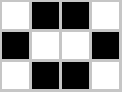
\includegraphics[height=.125\linewidth]{./images/beehive.png}
	\caption{Configuración inicial colmena.}
	\label{fig:beehive}
\end{figure} 
\begin{figure}[H]
	\centering
	
\includegraphics[height=.15\linewidth]{./images/beehive_with_tail.png}
	\caption{Configuración inicial colmena con cola.}
	\label{fig:beehive_tail}
\end{figure} 
\begin{figure}[H]
	\centering
	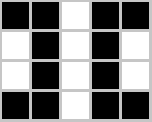
\includegraphics[height=.15\linewidth]{./images/table_on_table.png}
	\caption{Configuración inicial mesa frente a mesa.}
	\label{fig:table_on_table}
\end{figure} 

\begin{defi}
Una vida pseudo inmóvil es una vida inmóvil que puede ser particionada en vidas inmóviles independientes, es decir, la estabilidad de una de ellas no depende de la presencia de las otras. Además debe de existir al menos una célula muerta por superpoblación (más de tres vecinos vivos) que al particionar en vidas inmóviles independientes la célula continúe muerta por soledad (menos de tres vecinos vivos).
\end{defi}

Las vidas inmóviles que particionan a una vida pseudo inmóvil pueden ser a su vez vidas pseudo inmóviles \ref{fig:bisnake} o vidas inmóviles estrictas \ref{fig:biblock}. Notar que una vida inmóvil puede estar formada por varias vidas inmóviles y aún así ser una vida estrictamente inmóvil (y no pseudo inmóvil), si éstas dependen entre sí para mantener su estabilidad \ref{fig:table_on_table}.

\begin{figure}[H]
	\centering
	
\includegraphics[height=.125\linewidth]{./images/biblock.png}
	\caption{Configuración inicial bibloque.}
	\label{fig:biblock}
\end{figure} 

\begin{figure}[H]
	\centering
	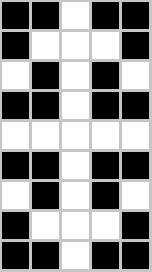
\includegraphics[height=.3\linewidth]{./images/bisnake.png}
	\caption{Configuración inicial que puede ser particionada en dos vidas pseudo inmóviles.}
	\label{fig:bisnake}
\end{figure} 


\begin{defi}
Una vida quasi inmóvil es una vida inmóvil que puede ser particionada en vidas inmóviles independientes, es decir, la estabilidad de una de ellas no depende de la presencia de las otras. Además existen células que tanto en la configuración inicial como en las vidas inmóviles independientes se mantengan muertas por soledad (menos de tres vecinos vivos). 
\end{defi}

Notar que la figura \ref{fig:biblock} no es una vida quasi inmóvil y sin embargo \ref{fig:bimoved} sí. Este tipo de vida inmóvil está habitualmente formada por dos vidas inmóviles que comparten una diagonal.

\begin{figure}[H]
	\centering
	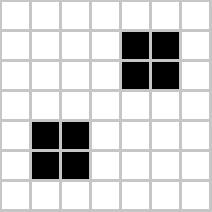
\includegraphics[height=.2\linewidth]{./images/bimoved.png}
	\caption{Configuración inicial que en el centro tiene una célula que se mantiene muerta por soledad tanto en las vidas inmóviles independientes como en el total.}
	\label{fig:bimoved}
\end{figure} 

Por último, cabría preguntarse el problema de dado un número finito de células, ¿cuántas vidas inmóviles existen? Dicho problema ha sido resuelto para vidas inmóviles estrictas y pseudo inmóviles de hasta 32 células, como se puede consultar en \cite{countStillLifes} y en \cite{countPseudoStillLifes}.

\subsection{Osciladores}

\begin{defi}
Un oscilador es una configuración inicial $z$ finita y no vacía que se repite tras la aplicación de $k$ veces de la función de transición global, esto es, fijado $n\in\mathds{N}$, se verifica que existe $k>1, \in\mathds{N}$ tal que $C^n_t(z) = C^n_{t+k}(z)$ para todo $t \leq n-k$ y diremos que $k$ es el periodo del oscilador.
\end{defi}

Notar que se exige que el periodo de oscilación sea estrictamente superior a la unidad, para evitar que la categoría de las vidas inmóviles esté contenidas dentro de la de los osciladores. 

\begin{figure}[H]
	\centering
	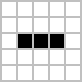
\includegraphics[height=.125\linewidth]{./images/blinker.png}
	\caption{El oscilador más pequeño de periodo dos.}
	\label{fig:blinker}
\end{figure} 

\subsection{Naves espaciales}

\begin{defi}
Una  nave espacial es una configuración inicial $z$ finita y no vacía que se repite tras la aplicación de $k$ veces de la función de transición global pero en una posición distinta, esto es, fijado $n\in\mathds{N}$, se verifica que existen $k\in\mathds{N}$ y una traslación distinta de la identidad, $\phi:\mathds{Z}^2\to\mathds{Z}^2$, tal que $C^n_t(z) = \phi(C^n_{t+k}(z))$ para todo $t \leq n-k$ y diremos que $k$ es el periodo de la nave espacial.
\end{defi}

Notar que se exige que la traslación $\phi$ sea distinta a la identidad y $k>1$, para evitar que la categoría de los osciladores esté contenida dentro de la de las naves espaciales.

Si la configuración se desplaza $x$ unidades horizontalmente e $y$ unidades verticalmente cada periodo de longitud $k$ la velocidad de desplazamiento de la nave espacial es $\max\{|x|,|y|\}c/k$ con pendiente $x/y$, siendo la velocidad máxima teórica conocida como \textit{velocidad de la luz} $c=1$, esto es, un desplazamiento por cada aplicación de la función de transición global. Según \cite{pendienteNaves} existe una nave espacial en el juego de vida de Conway para cada pendiente racional.

\begin{figure}[H]
	\centering
	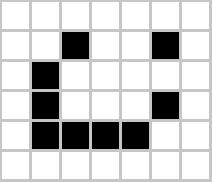
\includegraphics[height=.15\linewidth]{./images/lightweightspaceship.png}
	\caption{Nave espacial más pequeña conocida de velocidad $c/2$, su desplazamiento es paralelo a uno de los ejes de coordenadas cartesianos.}
	\label{fig:lightweightspaceship}
\end{figure} 
\begin{figure}[H]
	\centering
	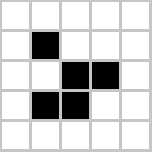
\includegraphics[height=.15\linewidth]{./images/glider.png}
	\caption{Nave espacial más pequeña conocida de velocidad $c/4$, su desplazamiento es diagonal a los ejes cartesianos de coordenadas.}
	\label{fig:glider}
\end{figure} 

\subsection{Características medidas sobre las simulaciones}

Dado el carácter aleatorio del juego de vida $\alpha$-asíncrono emplearemos los fundamentos de Monte Carlo expuestos en la sección \ref{MonteCarlo} para medir los parámetros de interés que a continuación expondremos. Dada una configuración inicial $z$ de las categorías expuestas en la sección \ref{zoo}, realizaremos múltiples simulaciones del juego de vida de Conway $\alpha$-asíncrono de duración $n=100$. Nuestras variables de interés son:

\begin{itemize}
\item Crecimiento de la población de células de la configuración inicial: dispondremos de dos herramientas para medir el número de células. Estudiaremos la evolución del número de células en cada etapa y la evolución del rectángulo de menor tamaño que contenga a todas las células de cada etapa.
\item Tasa de cambio de la configuración inicial: emplearemos el concepto de temperatura, que es el porcentaje medio el número de células que nacen o mueren por generación.
\item Distribución de las células en cúmulos: contabilizaremos el número de cúmulos por cada generación, entendiendo por cúmulo al mayor conjunto de células cuyo vecindario no es disjunto, es decir, en un cúmulo cada célula del mismo está contenido en el vecindario de otra célula del cúmulo.
\end{itemize}

Estas variables serán medidas para distintos valores de $\alpha$ con el fin de estudiar el efecto de la aleatoriedad en las configuraciones iniciales. Notar que debido a que no se conoce a priori el número de simulaciones a partir de la cual es posible aplicar el teorema central del límite para deducir la distribución límite de la suma de variables aleatorias, el número de simulaciones que realizaremos podrá variar de una configuración inicial a otra.

% Características a medir si sobra tiempo: simulaciones utilizando cadenas de markov y métodos de monte carlo


